\providecommand{\myrootdir}{..}
\documentclass[\myrootdir/main.tex]{subfiles}

\begin{document}

\chapter{Empirical Comparison}
\label{sec:study}
To investigate when PBE, CTS and KWS are suited to retrieve chunks from CI build logs we evaluate them on the \emph{LogChunks} data set.
This chapter describes our study design, detailing which metrics we measure to answer our research questions.
In the presentation of the results, we first focus on each of the three techniques and later compare them against each other.


\begin{figure}[htbp]
	\centering
	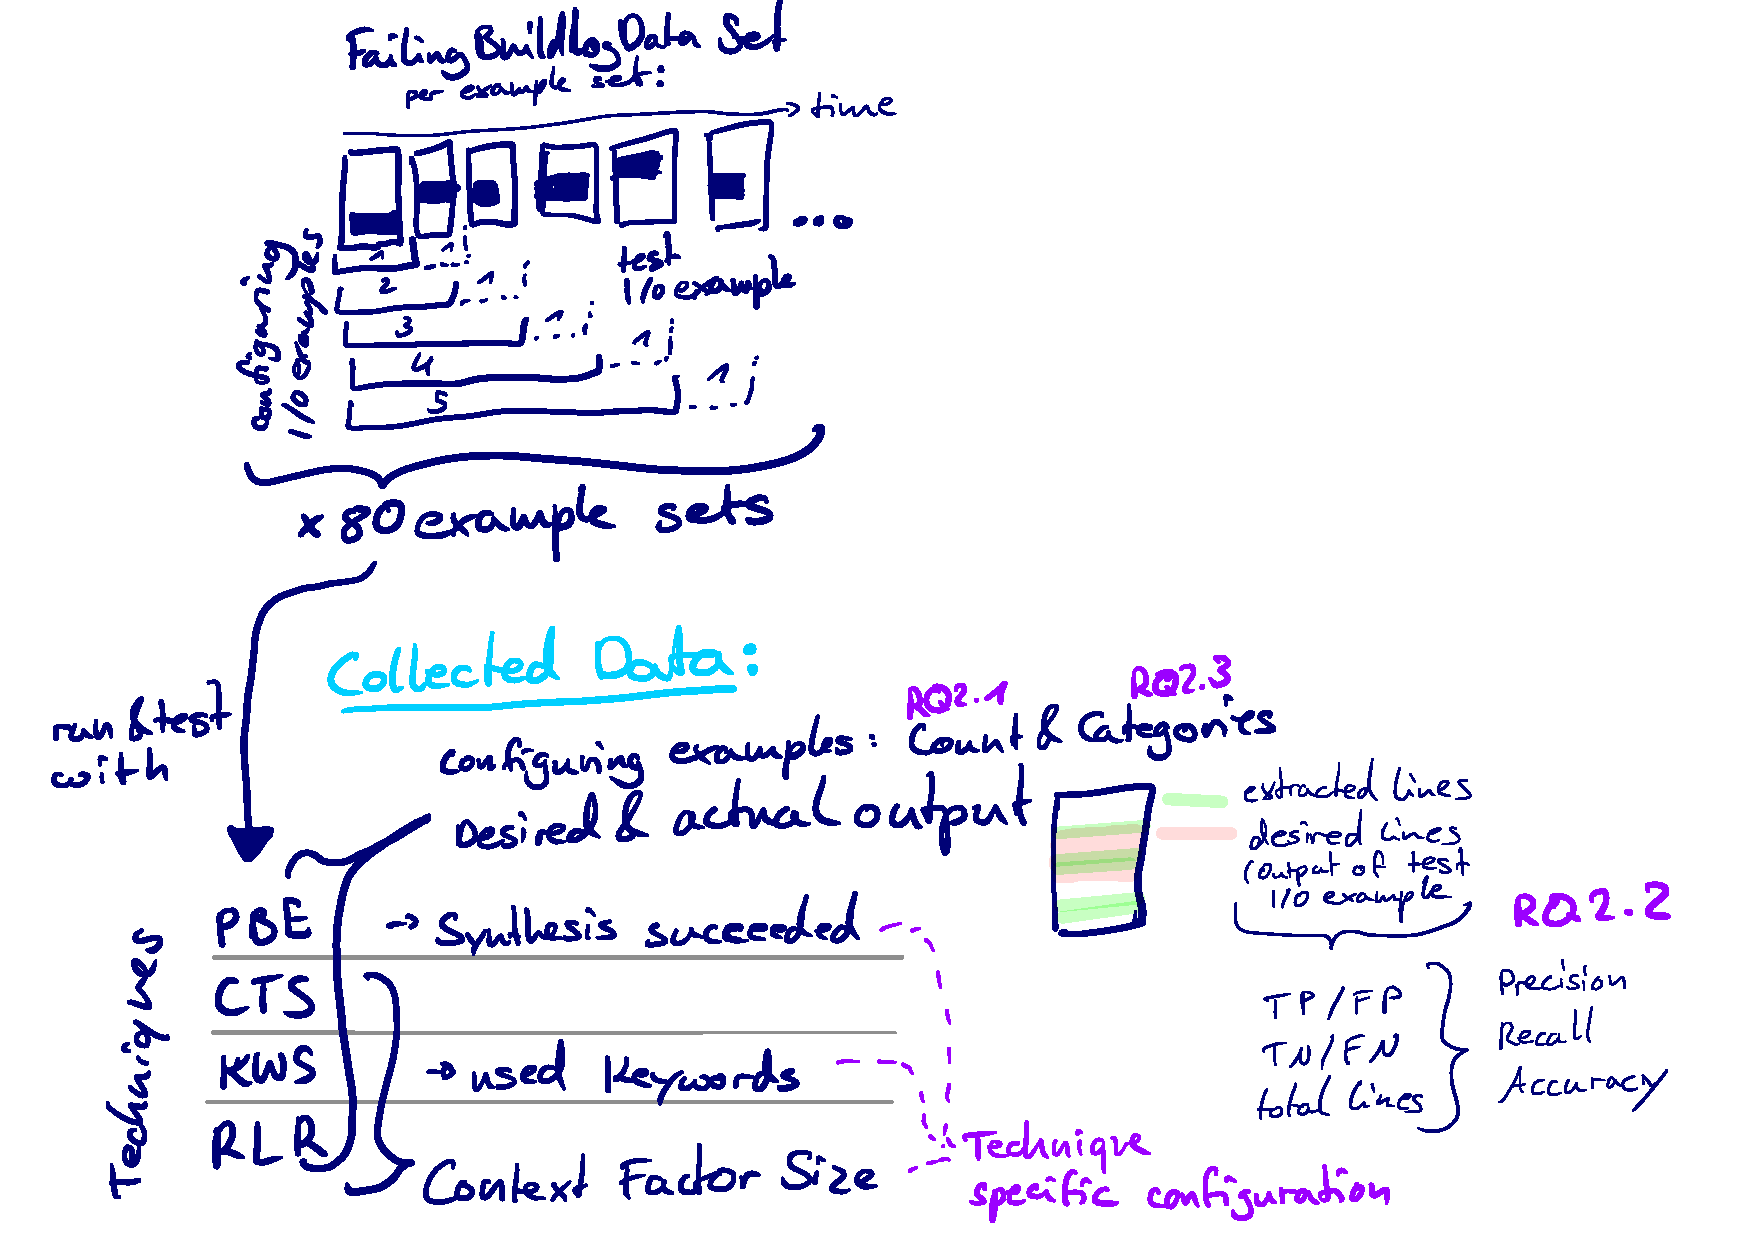
\includegraphics[width=\textwidth, clip]{img/study-design.pdf}
	\caption{Study design of our technique comparison study}
	\label{fig:study}
\end{figure}


\begin{simplebox}{Research Questions}
\begin{itemize}
  \item[\textbf{RQ1:}] Which criteria influence the suitability of a chunk retrieval technique for CI build logs?
  \item[\textbf{RQ2:}] Under which conditions are PBE, CTS, and KWS suited to retrieve information from CI build logs?
  \item[\textbf{RQ2.1:}] How many examples do PBE, CTS, and KWS need to perform best?
  \item[\textbf{RQ2.2:}] How structurally similar do the examples for PBE, CTS and KWS need to be for the techniques to be applicable?
  \item[\textbf{RQ2.3:}] How accurate are the retrievals of PBE, CTS, and KWS?
\end{itemize}
\end{simplebox}

\section{Study Design}
For the comparison, we evaluate the three chunk retrieval techniques PBE, CTS and KWS, described in Sections~\ref{sec:expl-pbe},\ref{sec:expl-ts} and~\ref{sec:expl-skws}.
RLR, explained in Section~\ref{sec:expl-rlr}, acts as a baseline for the comparison.
We run four techniques on the Examples from \emph{LogChunks}.

\paragraph{Training and Test Set}
The data set for this study are the examples from \emph{LogChunks}.
They contain build logs, the substring describing the reason the build failed, keywords to search for that substring and which structural category the substring belongs to.

For each repository in \emph{LogChunks}, we split the examples chronologically into training and test set.
Therefore we train on examples from past build logs and test on future build logs.

\paragraph{RQ 2.1: Size of Training and Test Set}
To analyze how many examples the chunk retrieval techniques need to perform best, we evaluate the techniques with different training set sizes.
We run each technique with one to five examples from each repository within \emph{LogChunks}.
The size of the test set is one.

\paragraph{RQ 2.2: Recording Structural Categories}
To determine how structurally similar the examples for the chunk retrieval techniques need to be, we record the structural categories of the examples in the training and test sets.

\paragraph{RQ2.3: Accuracy Metrics}
To measure the accuracy of the retrieved chunks we save the actual output lines of each chunk retrieval run ($retrievedlines$).
As oracle in our evaluation, we save the desired lines from the output of the test example ($desiredlines$).
We calculate the following metrics:
\begin{itemize}
	\item \todo{FILL}
	\item True positives: $TP = desiredlines \cap retrievedlines$
	\item False positives: $FP = retrievedlines - desiredlines$
	\item True negatives: $TN = allloglines - (retrievedlines \cup desiredlines)$
	\item False negatives: $FN = desiredlines - retrievedlines$
	\item Precision: $Precision = TP / retrievedlines$
	\item Recall: $Recall = TP / desiredlines$
	\item F-Score:
	\item Successful Extraction: $true if Recall == 1$
\end{itemize}

% The examples are sorted chronologically, i.e.\ a technique is configured with examples from the directly preceding build logs.
% For each example set and each technique, we select one to five consecutive I/O examples as configuration, the \emph{training examples}, and run the chunk retrieval on the following I/O example, the \emph{test example}.

% For each of our evaluation runs we measure the desired and the actual output lines of the chunk retrieval.
% The desired output is given by the output of the test example, which acts as the oracle for our evaluation.
% From this we obtain true/false positives/negatives and calculate precision, recall and accuracy.
% We use these values to answer \textbf{RQ2.2}.
% If all desired lines are extracted, i.e.\ recall is one, we say a chunk retrieval run was \emph{successful}.
% To answer \textbf{RQ2.1}, we register the number training examples for each run.
% The structural categories of the training examples are saved to answer \textbf{RQ2.3}.
Recall and precision of CTS and KWS vary with the number of lines selected for retrieval.
We evaluate the effect of varying the number of extracted lines by multiplying the average number of lines present in the training examples with a \emph{retrieval size factor} from 0.5 to 2.5 in steps of 0.5.

%taking The LogChunks data Set - run 3(4 with random) techniques with increasing example count - measuring xyz - justify choices like running chronologically / testing on 1 example / no k-fold validation - how are keywords for the search selected?

\section{Results}
This section presents the results for PBE, CTS and KWS separately.
Afterwards we compare the three techniques with each other and RLR as baseline.

% \begin{figure}[htbp]
% 	\centering
% 	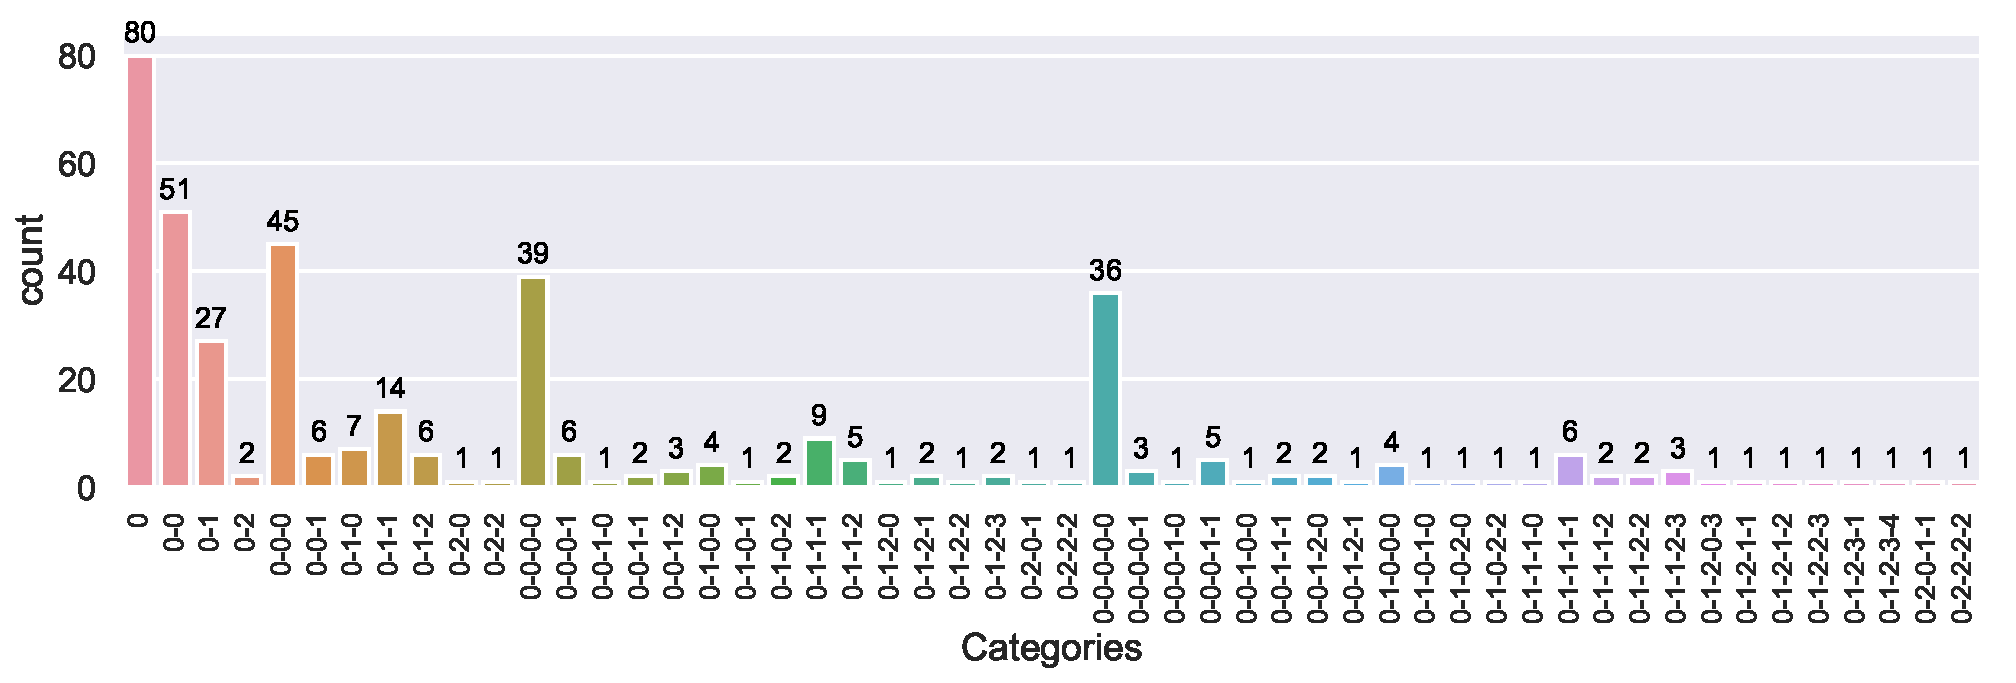
\includegraphics[width=\textwidth, clip]{img/big-study/categories-dataset.pdf}
% 	\caption{Distribution of Category Combinations in the Example Sets used for Configuration in our Study}
% 	\label{fig:categories-dataset}
% \end{figure}

% \begin{figure}[htbp]
% 	\centering
% 	\begin{minipage}{0.45\textwidth}
% 		\centering
% 		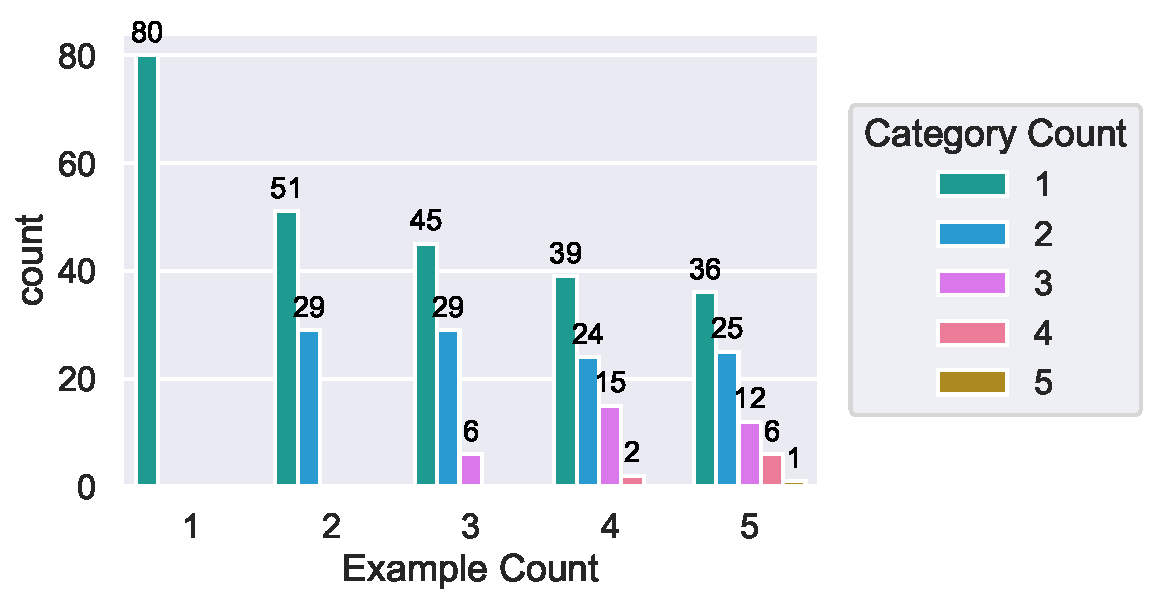
\includegraphics[width=\textwidth, clip]{img/big-study/categorycount-examplecount-dataset.pdf}
% 		\caption{Distribution of the Count of Categories within the Examples used for Configuration in our Study}
% 		\label{fig:categorycount-examplecount-dataset}
% 	\end{minipage}\hfill
% 	\begin{minipage}{0.45\textwidth}
% 		\centering
% 		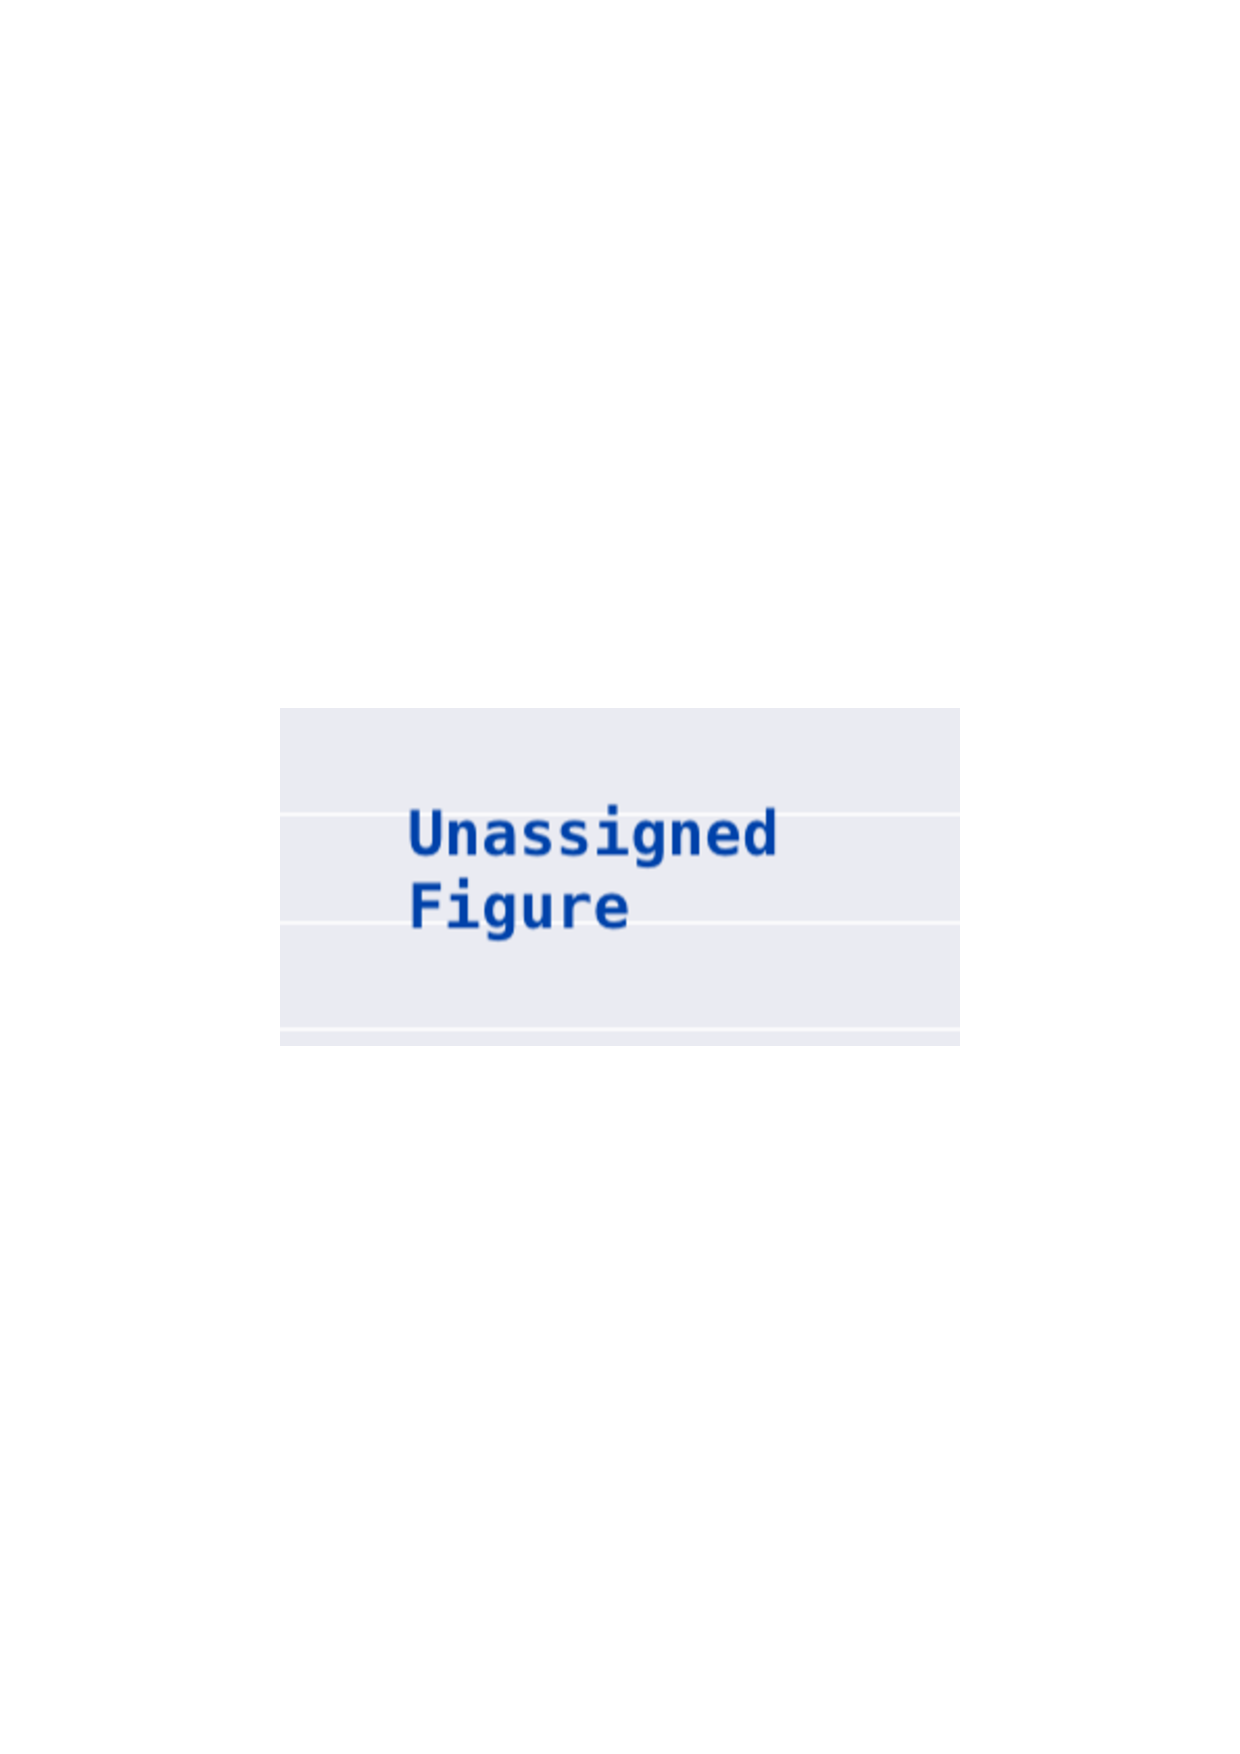
\includegraphics[width=\textwidth, clip]{img/big-study/xxx.pdf}
% 		\caption{caption}
% 		\label{fig:xxxy}
% 	\end{minipage}
% \end{figure}

% \subsection{Category Distribution in Data Set}
% Categories distributed in over data set
% - why are we looking at that?: interesting how categories are distributed for this real world example of build Failure reasons in travis ci categorization
% - Figure~\ref{fig:categories-dataset} shows the distribution of categories in the configuring example sets in rou study
% - Figure~\ref{fig:categorycount-examplecount-dataset} shows the category count separated by the different example count.

\begin{figure}[htbp]
		\centering
		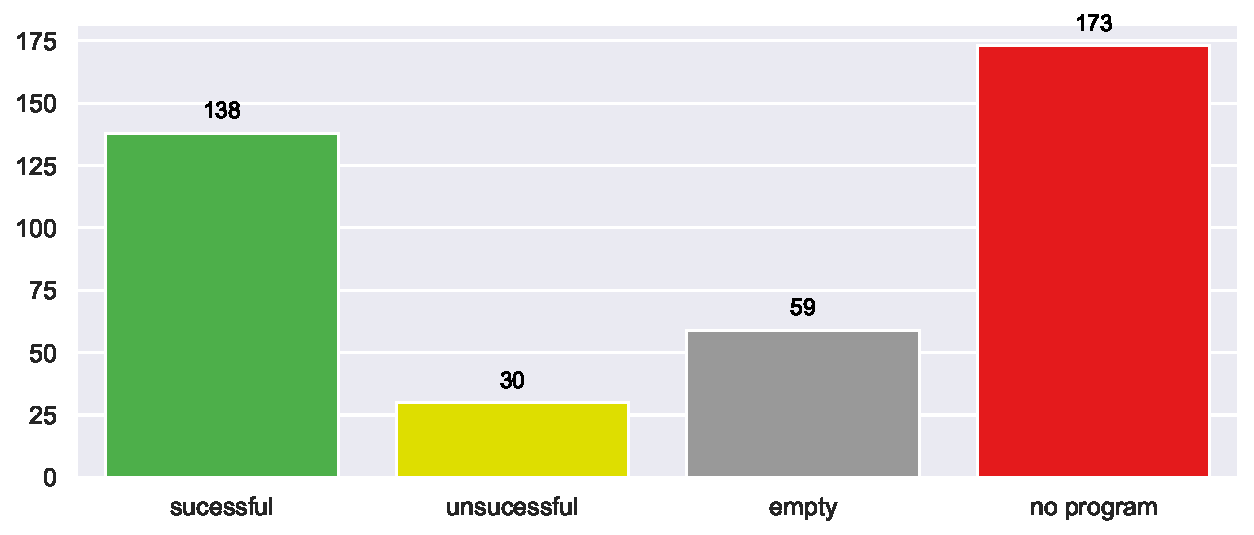
\includegraphics[width=\textwidth, clip]{img/big-study/failure-reason-PBE.pdf}
		\caption{Results of chunk retrieval with PBE}
		\label{fig:failure-reason-PBE}
\end{figure}

\begin{figure}[htbp]
		\centering
		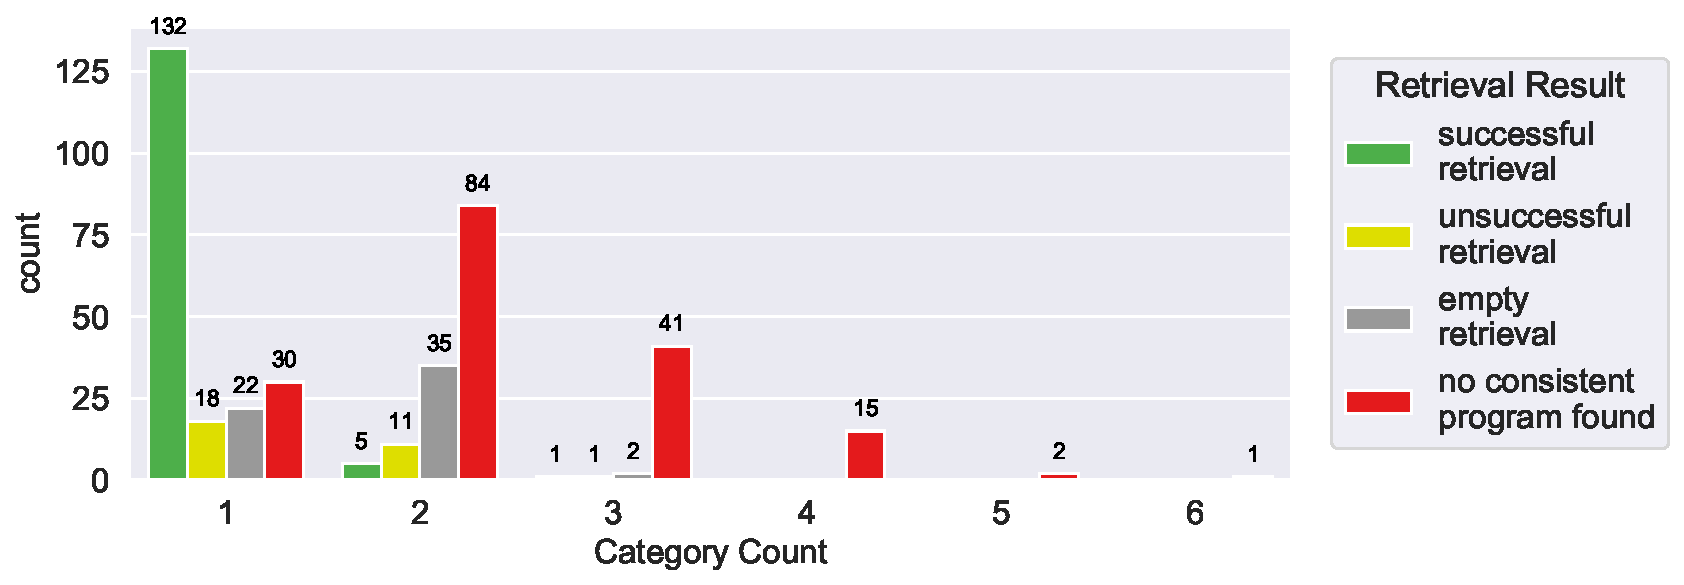
\includegraphics[width=\textwidth, clip]{img/big-study/failure-reason-categorycount-PBE.pdf}
		\caption{Results of chunk retrieval with PBE for increasing number of structural categories in the training set}
		\label{fig:failure-reason-categorycount-PBE}
\end{figure}

\begin{figure}[htbp]
		\centering
		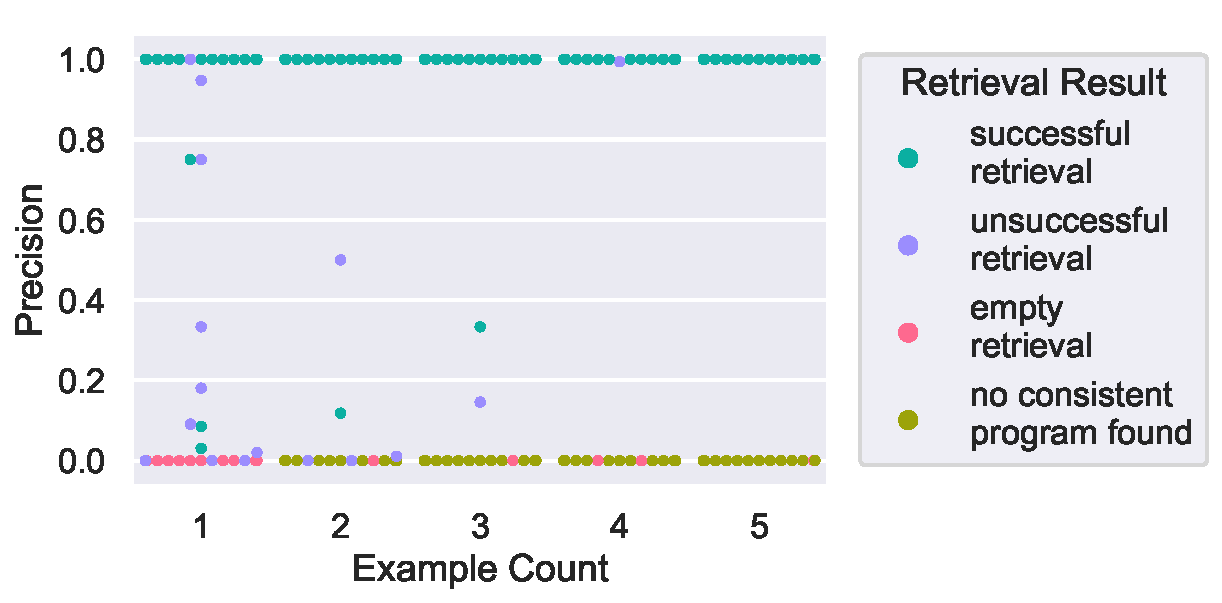
\includegraphics[width=\textwidth, clip]{img/big-study/precision-extraction-result-PBE.pdf}
		\caption{Precision of chunk retrieval with PBE for increasing training set size}
		\label{fig:precision-extraction-result-PBE}
\end{figure}

\subsection{Program Synthesis by Example (PBE)}
Figure~\ref{fig:failure-reason-PBE} shows the results of the PBE runs in our evaluation.
Out of the 400 runs, 5 per each one of the 80 example sets, PBE extracted all the desired lines in 138 cases.
Figure~\ref{fig:failure-reason-PBE} shows that in 89 further cases a program was also successfully synthesized, though in 59 cases the synthesized program yielded no output at all.
In 30 cases the synthesized program did not extract all of the desired lines, though still had an average recall of 28\%.
In 173 cases the PROSE program synthesis could not synthesize a singular regular expression program that satisfies all of the training examples.

Figure~\ref{fig:failure-reason-categorycount-PBE} shows the results of PBE runs compared to the number of structural categories present in the training examples.
It shows that the program synthesis is more likely to succeed when there are few categories present in the training examples.
When two structural categories are present, PROSE could in most cases not synthesize a program consistent with all training examples.
For three or more present categories PROSE could never synthesize a consistent program.

Figure~\ref{fig:precision-extraction-result-PBE} compares the precision of the PBE chunk retrieval runs with the training set size.
For one example there is a high number of empty extraction outputs, meaning that the regular expression synthesized from this one training example could not be applied to the test example.
For two or more I/O examples the chunk retrieval is in most cases either successful or no consistent program could be synthesized.


\begin{figure}[htbp]
		\centering
		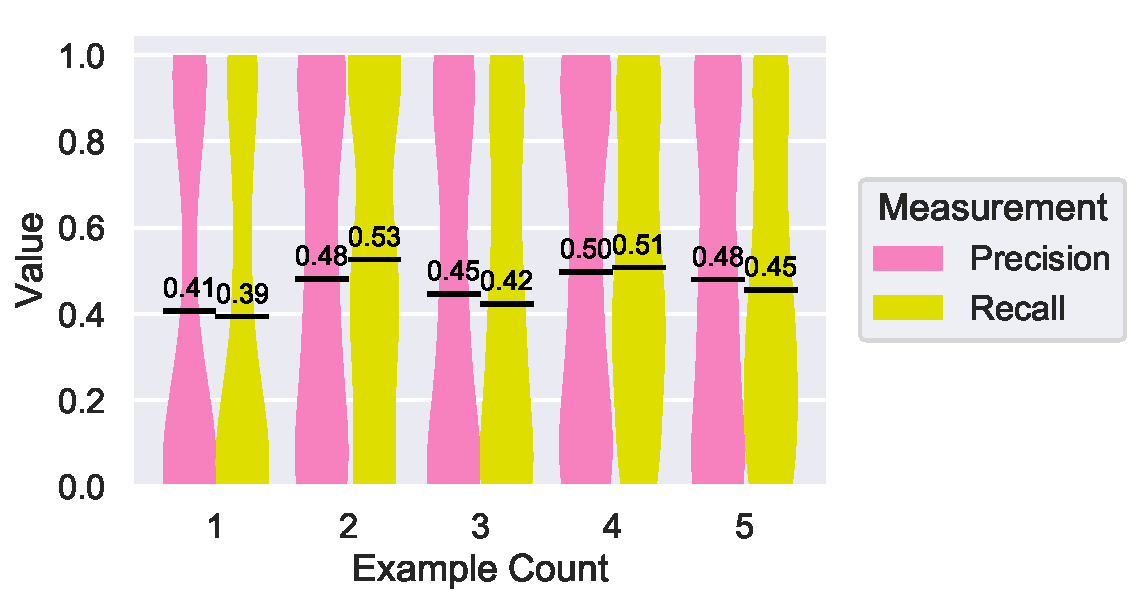
\includegraphics[width=\textwidth, clip]{img/big-study/recall-precision-examplecount-CTS.pdf}
		\caption{Precision and recall of chunk retrieval with CTS for increasing training set size}
		\label{fig:recall-precision-examplecount-CTS}
\end{figure}

\begin{figure}[htbp]
		\centering
		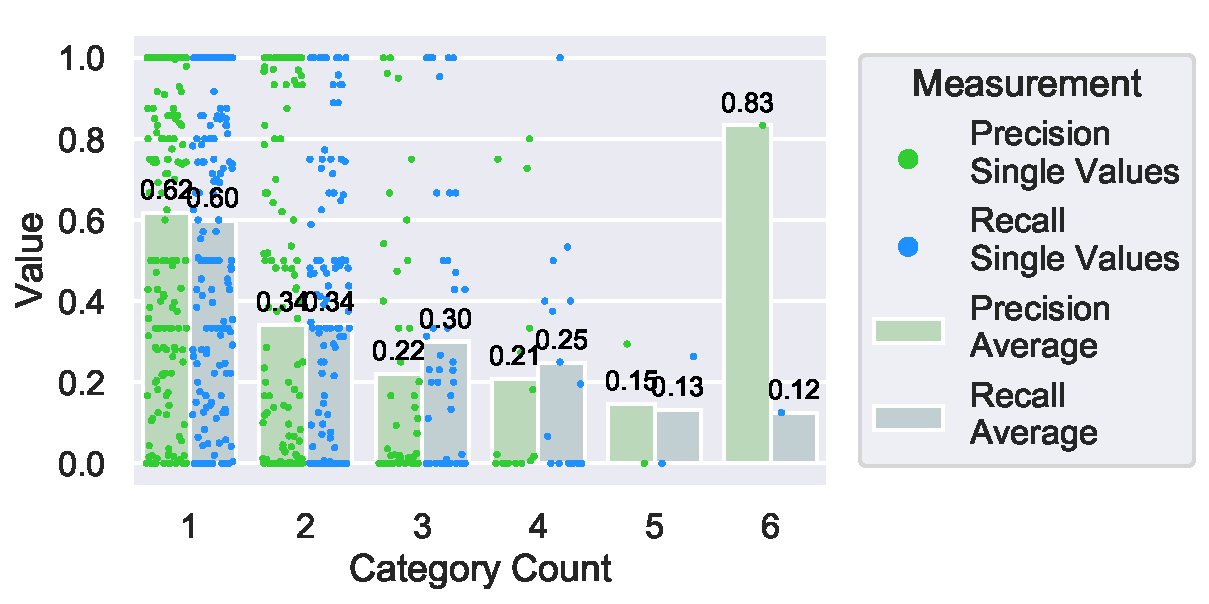
\includegraphics[width=\textwidth, clip]{img/big-study/recall-precision-categorycount-CTS.pdf}
		\caption{Precision and recall of chunk retrieval with CTS for increasing number of structural categories in the training set}
		\label{fig:recall-precision-categorycount-CTS}
\end{figure}

\begin{figure}[htbp]
		\centering
		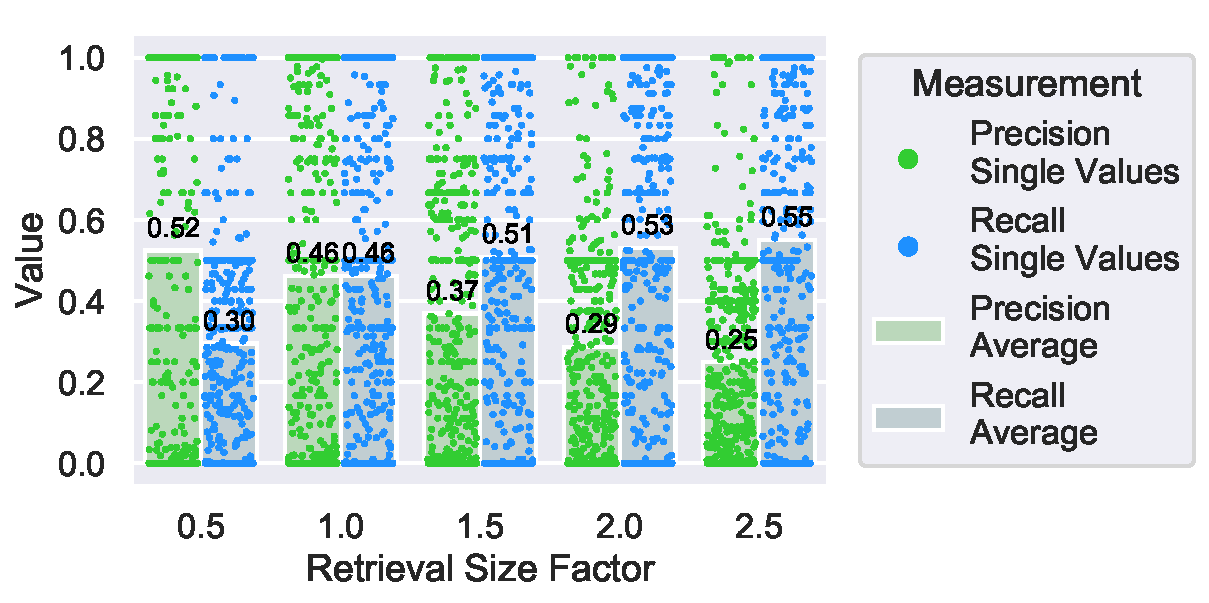
\includegraphics[width=\textwidth, clip]{img/big-study/contextsizefactor-precision-recall-CTS.pdf}
		\caption{Precision and recall of chunk retrieval with CTS compared to retrieval size factors}
		\label{fig:contextsizefactor-precision-recall-CTS}
\end{figure}

\subsection{Common Text Similarity (CTS)}
Figure~\ref{fig:recall-precision-examplecount-CTS} presents precision and recall of chunk retrieval using CTS for increasing training set size.
The size of the training set has no visible influence on recall and precision of the chunk retrieval with CTS\@.

Figure~\ref{fig:recall-precision-categorycount-CTS} shows the same measurements for different category counts in the training examples.
With increasing category count, precision and recall decrease.
Especially for more than three categories present we have no chunk retrieval runs where all desired lines were extracted.

Figure~\ref{fig:contextsizefactor-precision-recall-CTS} shows the effect of the retrieval size factor on precision and accuracy of chunk retrieval runs with CTS\@.
The precision ranges from 52\% when retrieving half expected number of lines to 25\% when 2.5 times the expected number of lines.
The recall ranges from 30\% to 55\%.


\begin{figure}[htbp]
		\centering
		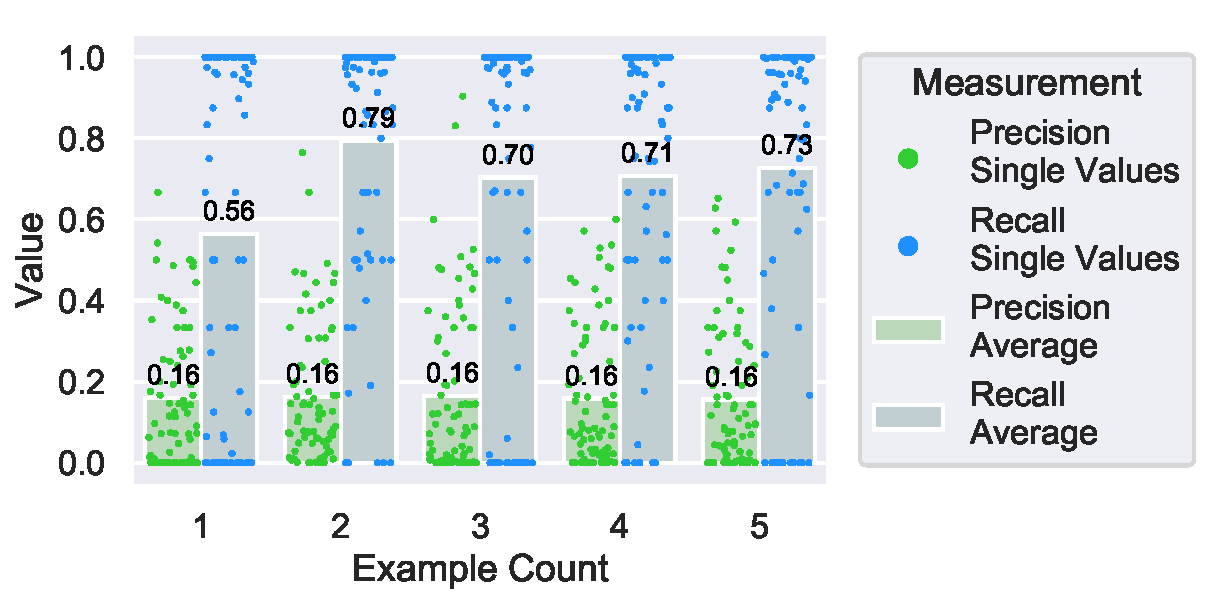
\includegraphics[width=\textwidth, clip]{img/big-study/recall-precision-examplecount-KWS.pdf}
		\caption{Precision and recall of chunk retrieval with KWS for increasing training set size}
		\label{fig:recall-precision-examplecount-KWS}
\end{figure}

\begin{figure}[htbp]
		\centering
		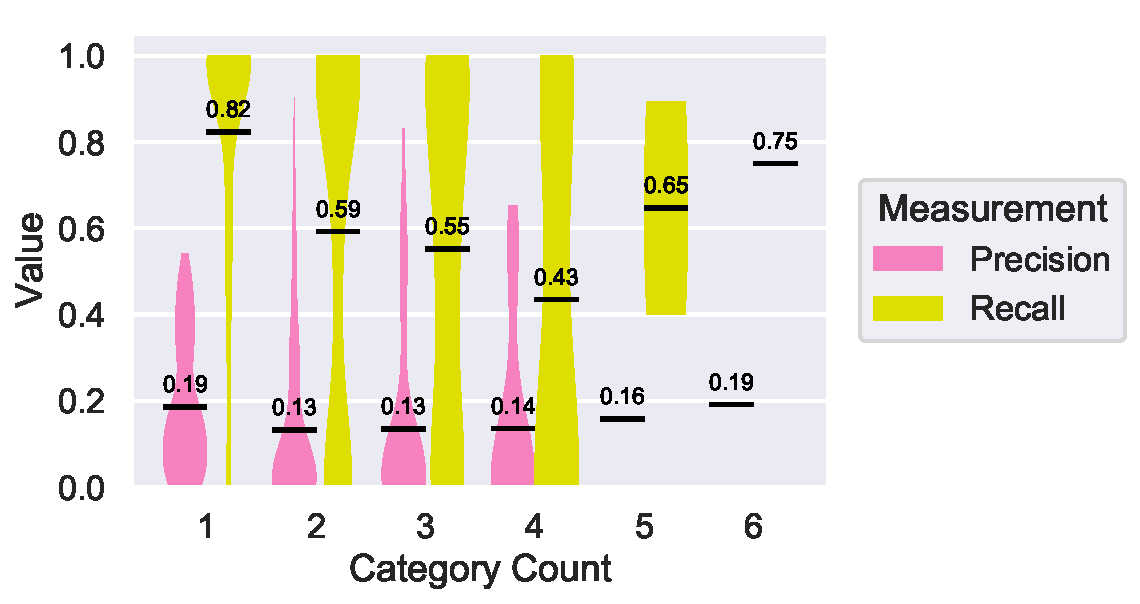
\includegraphics[width=\textwidth, clip]{img/big-study/recall-precision-categorycount-KWS.pdf}
		\caption{Precision and recall of chunk retrieval with KWS for increasing number of structural categories in the training set}
		\label{fig:recall-precision-categorycount-KWS}
\end{figure}

\begin{figure}[htbp]
		\centering
		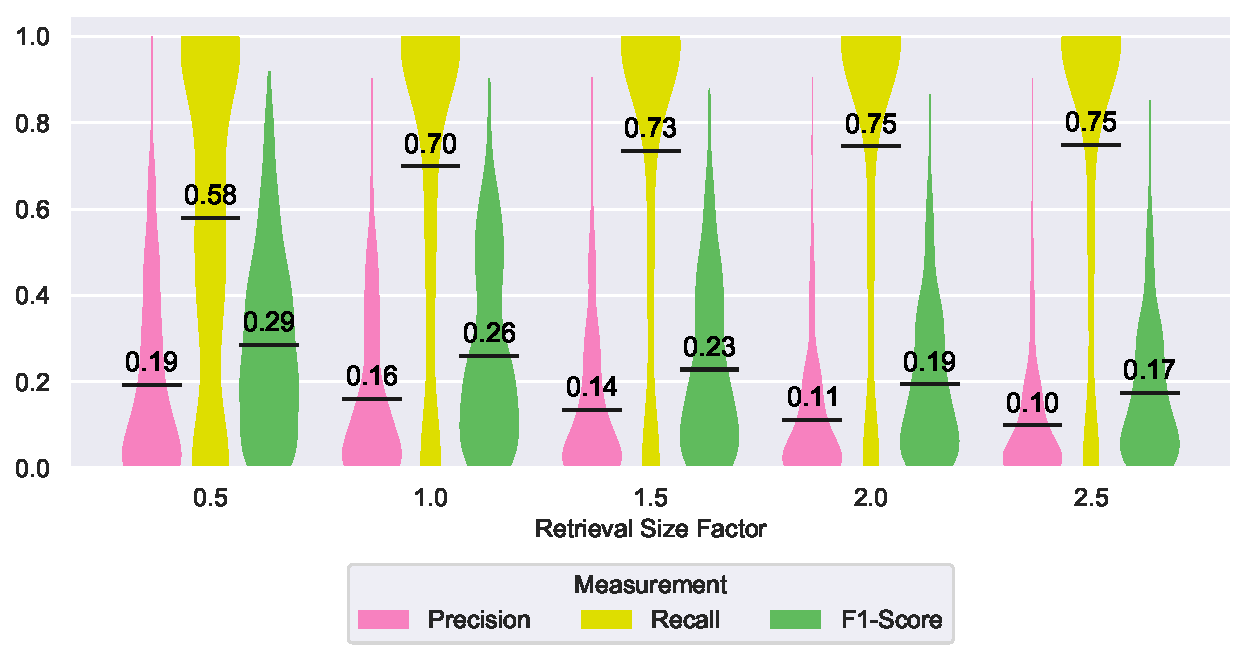
\includegraphics[width=\textwidth, clip]{img/big-study/contextsizefactor-precision-recall-KWS.pdf}
		\caption{Precision and recall of chunk retrieval with KWS compared to retrieval size factor}
		\label{fig:contextsizefactor-precision-recall-KWS}
\end{figure}


\begin{figure}[htbp]
		\centering
		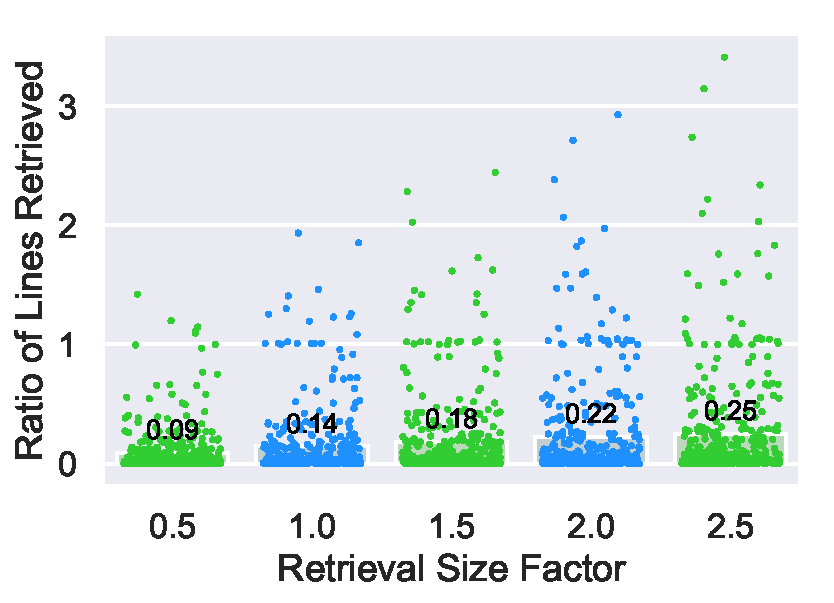
\includegraphics[width=\textwidth, clip]{img/big-study/retrievalsizefactor-retrievalratio-KWS.pdf}
		\caption{Ratio of lines retrieved with KWS compared to retrieval size factor}
		\label{fig:retrievalsizefactor-retrievalratio-KWS}
\end{figure}

\subsection{Keyword Search (KWS)}
Figure~\ref{fig:recall-precision-examplecount-KWS} presents precision and recall of chunk retrieval using KWS in our study for different numbers of training examples.
The recall increases by 12\% when increasing the size of the training set to more than one example, while the precision stays constant at around 16\%.

Figure~\ref{fig:recall-precision-categorycount-KWS} shows the same measurements for different category counts in the training examples.
There is no clear trend visible in precision and recall for an increasing amount of categories in the training examples

Figure~\ref{fig:contextsizefactor-precision-recall-KWS} shows the effect of the retrieval size factor on precision and accuracy of chunk retrieval runs with KWS\@.
The precision ranges from 19\% when retrieving half expected number of lines to 10\% when 2.5 times the expected number of lines.
The recall ranges from 58\% to 75\%.

Figure~\ref{fig:retrievalsizefactor-retrievalratio-KWS} shows the average proportion of the lines in the test log file retrieved for different retrieval size factors with KWS\@.
When retrieving the mean number of lines in the training examples, 15\% of the log lines are retrieved on average.
This proportion goes up to 25\% when retrieving 1.5 times more lines.

% \begin{figure}[htbp]
% 	\centering
% 	\begin{minipage}{0.45\textwidth}
% 		\centering
% 		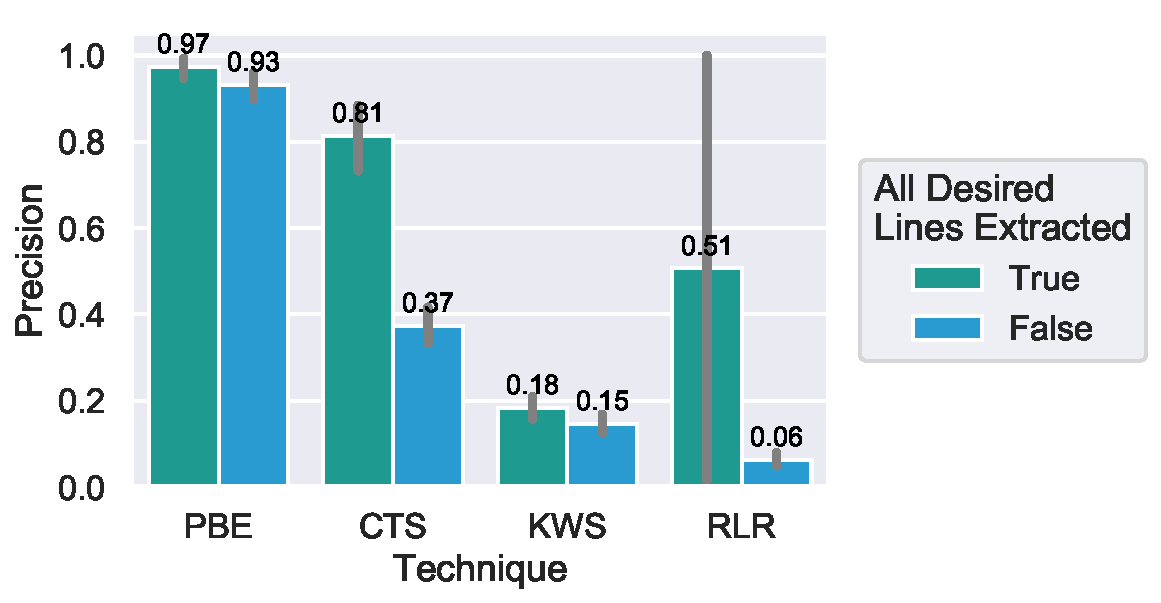
\includegraphics[width=\textwidth, clip]{img/big-study/precision-all.pdf}
% 		\caption{Precision \todo{and recall} of chunk retrieval with PBE, CTS and KWS compared with RLR}
% 		\label{fig:precision-all}
% 	\end{minipage}\hfill
% 	\begin{minipage}{0.45\textwidth}
% 		\centering
% 		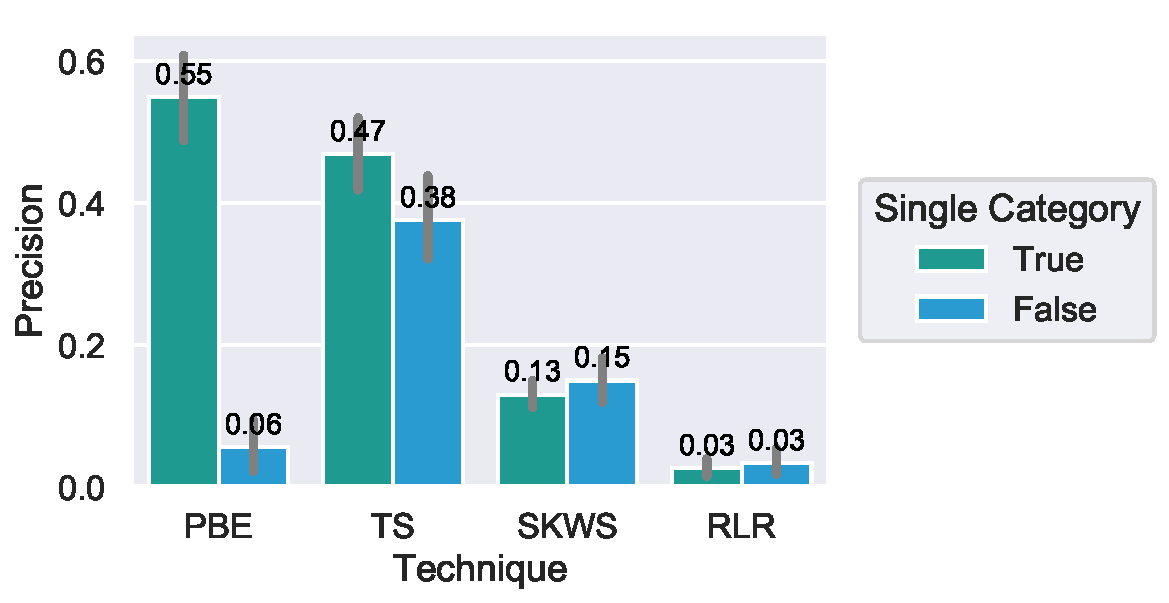
\includegraphics[width=\textwidth, clip]{img/big-study/precision-category-singularity-all.pdf}
% 		\caption{Precision \todo{and recall} of chunk retrieval with PBE, CTS and KWS compared with RLR for single and multiple categories present in the training examples}
% 		\label{fig:precision-category-singularity-all}
% 	\end{minipage}
% \end{figure}


\begin{figure}[htbp]
		\centering
		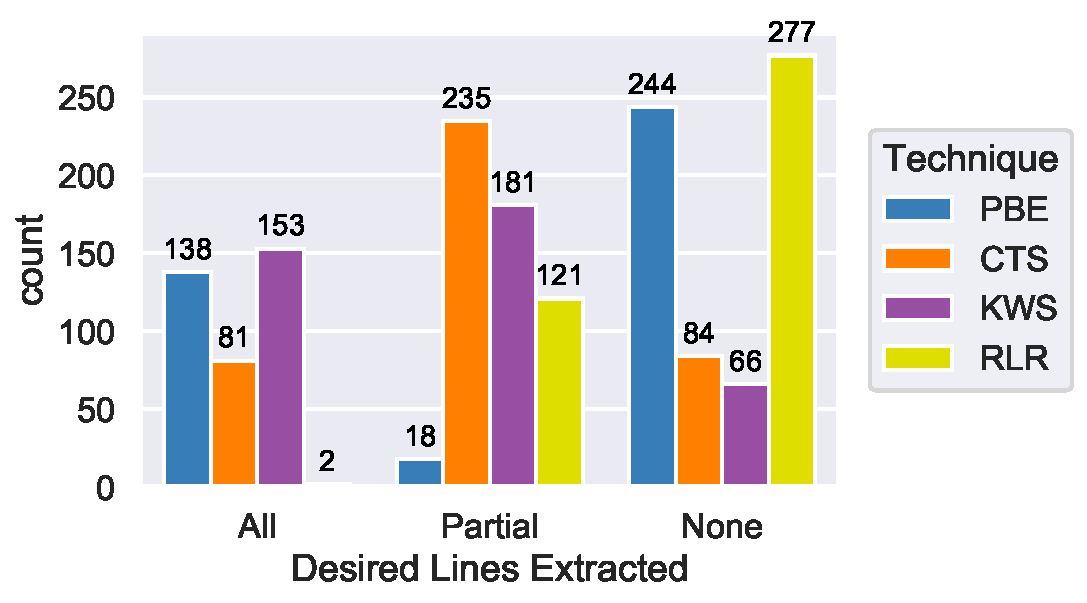
\includegraphics[width=\textwidth, clip]{img/big-study/success-partial-all.pdf}
		\caption{Success of chunk retrievals for all techniques}
		\label{fig:success-partial-all}
\end{figure}


\begin{figure}[htbp]
		\centering
		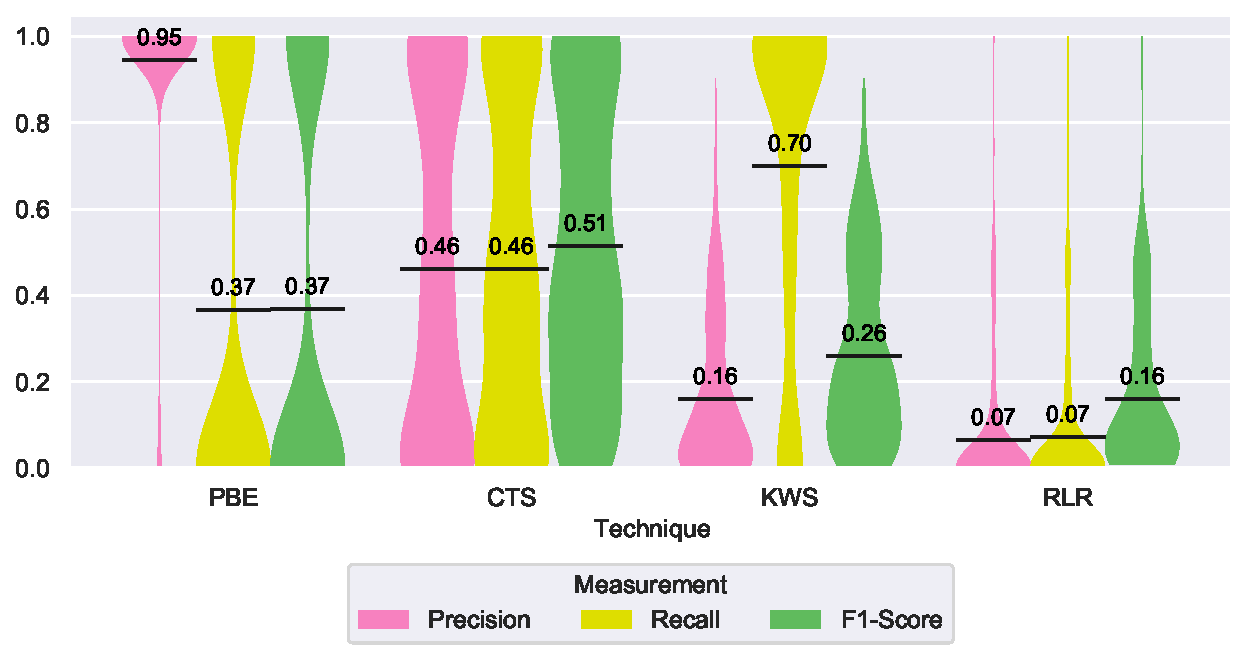
\includegraphics[width=\textwidth, clip]{img/big-study/recall-precision-all.pdf}
		\caption{Precision and Recall of all techniques compared}
		\label{fig:recall-precision-all}
\end{figure}

\begin{figure}[htbp]
	\centering
		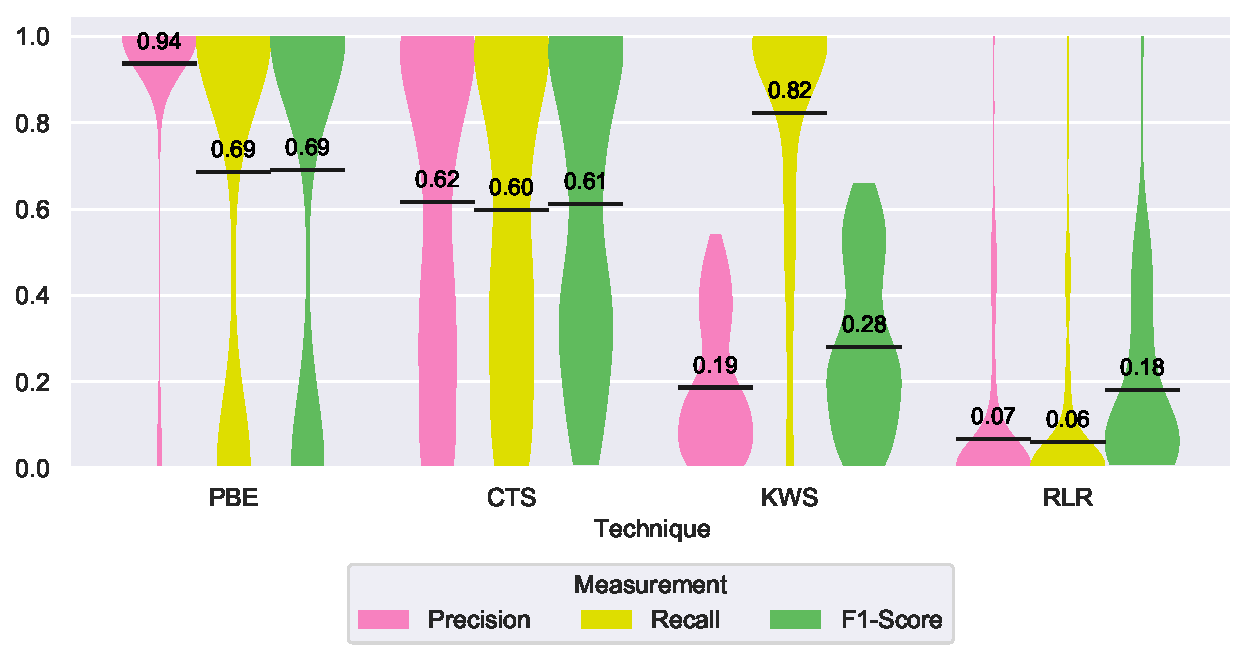
\includegraphics[width=\textwidth, clip]{img/big-study/recall-precision-singlecategory-all.pdf}
		\caption{Precision and Recall of all techniques compared when training examples are in \emph{one} structural category}
		\label{fig:recall-precision-singlecategory-all}
\end{figure}

\begin{figure}[htbp]
		\centering
		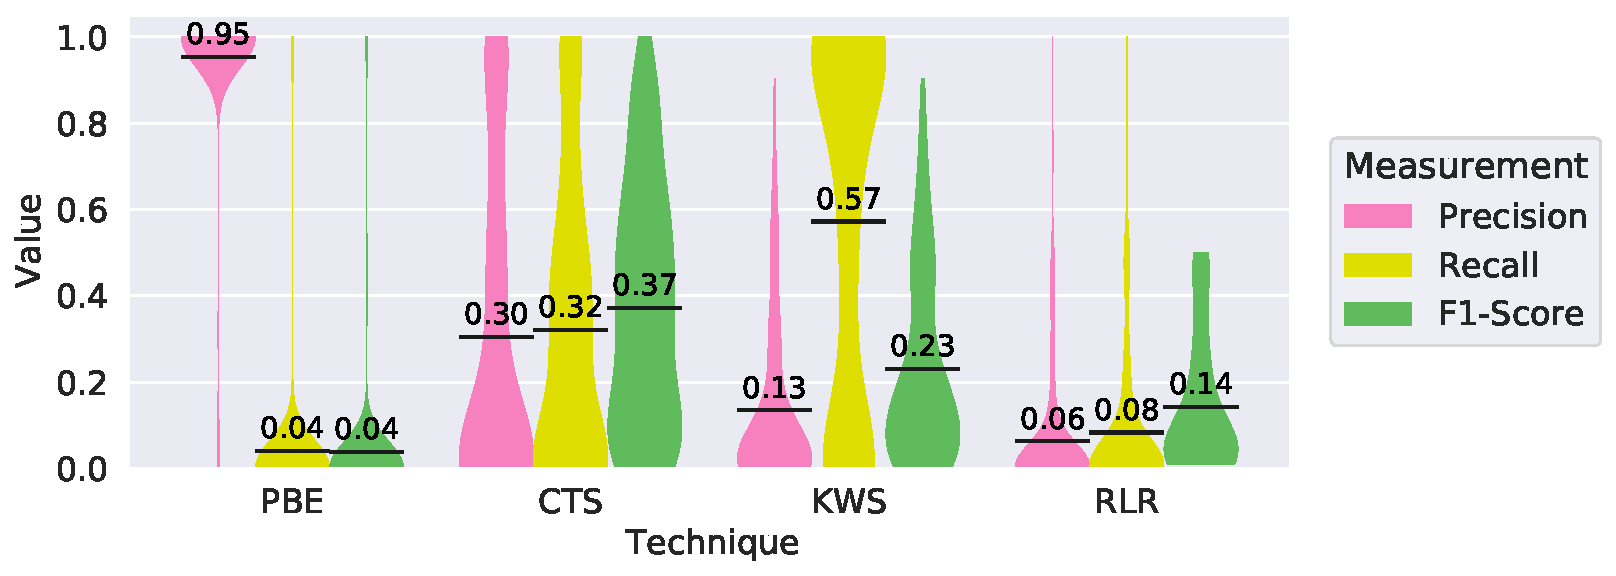
\includegraphics[width=\textwidth, clip]{img/big-study/recall-precision-multicategory-all.pdf}
		\caption{Precision and Recall of all techniques compared when training examples are in \emph{more than one} structural categories}
		\label{fig:recall-precision-multicategory-all}
\end{figure}

% \begin{table}[htbp]
% \centering
% \begin{tabular}{ |c||c|c|c| }
% 	\hline
%   Technique & \multicolumn{3}{|c|}{Desired Lines extracted} \\
%   \hline
%   & all [0.345 , 0.2025, 0.3825, 0.005 ] & partial [0.045 , 0.5875, 0.4525, 0.3025] & none [0.61  , 0.21  , 0.165 , 0.6925] \\
%   \hline
%   & recall = 1 & 0 < recall < 1 & recall = 0 \\
%   \hline
%   PBE & 138 & 18 & 244 \\ 
%   CTS & 81 & 235 & 84 \\ 
%   KWS & 153 & 181 & 66 \\ 
%   RLR & 2 & 121 & 277 \\ 
%   \hline
% \end{tabular}
% \caption{Comparison of successful extractions for PBE, CTS, KWS and RLR}
% \label{tab:101}
% \end{table}

\subsection{Comparison of All Techniques}
Figure~\ref{fig:success-partial-all} compares the success of all chunk retrieval of the different techniques in our study.
CTS and KWS extract at least some of the desired lines in 79\% and 88.5\%.
With 38.25\%, KWS also has the highest number of successful extractions, followed by PBE with 34.5\%.
PBE has the lowest number of partial extraction with only 18 out of 400 chunk retrieval runs.

The averaged precision and recall of all techniques is compared in Figure~\ref{fig:recall-precision-all}.
PBE has a high skew towards one and zero for both measurements, meaning in most cases either the retrieval is successful or no relevant lines are extracted at all.
Chunk retrieval with CTS has the highest average precision with 46\% and the second best recall with 45\%.
KWS has the smallest precision of the three chunk retrieval techniques.
With 16\% it is still higher than the precision of the RLR baseline with 7\%.
KWS has the highest recall of all techniques with 70\%.

Figure~\ref{fig:recall-precision-singlecategory-all} and Figure~\ref{fig:recall-precision-multicategory-all} show the influence of a single structural category present in the training examples compared to multiple categories present.
For more than one present category, precision and recall of PBE greatly decrease.
For CTS and KWS the values also decrease slightly, while RLR is not affected by the number of structural categories present.

\end{document}
